%%%%% Define Tikz colors and styles %%%%%

\definecolor{cores}{HTML}{173F5F}
\definecolor{kpar}{HTML}{3BAEA3}
\definecolor{npar}{HTML}{ED553B}

\tikzset{my lines/.style={
    black!30!white, line width = 0.2pt
}}

\tikzstyle{arrow} = [->, >=latex, very thick]
\tikzstyle{corebox} = [very thick, step=1, fill opacity=0.5]
\tikzstyle{connection} = [thick]

%%%%% TikZpicture %%%%%

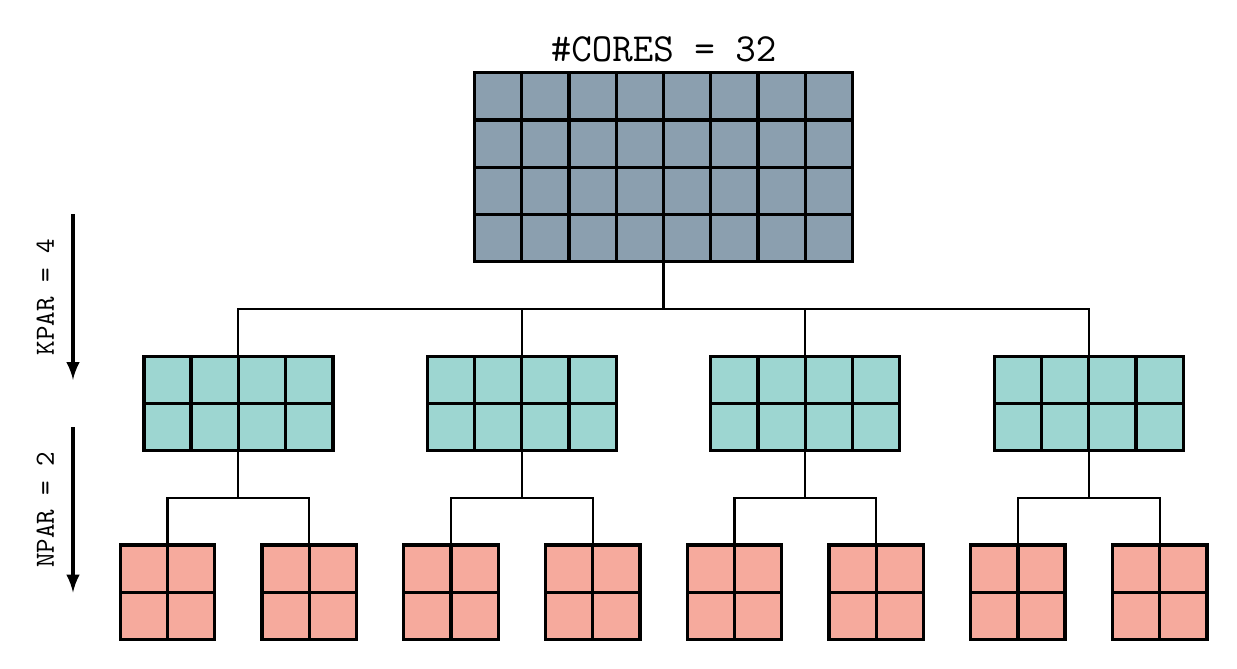
\begin{tikzpicture}[scale=0.6, node distance=0.4em]

% Draw the core boxes
\draw [corebox, xshift=0.5cm, fill=cores] (7, 8) grid (15, 12) rectangle (7, 8);
\foreach \x in {0, 6, ..., 21}
    \draw [corebox, xshift=0.5cm, fill=kpar] (\x, 4) grid (\x +4, 6) rectangle (\x, 4);
\foreach \x in {0, 3, ..., 21}
    \draw [corebox, fill=npar] (\x, 0) grid (\x + 2,2) rectangle (\x, 0) ;

% Draw connections
\draw [connection] (11.5, 8) -- (11.5, 7);
\foreach \x in {2.5, 8.5, ..., 21}
    \draw [connection] (11.5, 7) -- (\x, 7) -- (\x, 6);
    
\foreach \x in {2.5, 8.5, ..., 21}{
    \draw [connection] (\x, 4) -- (\x, 3);
    \draw [connection] (\x, 3) -- (\x - 1.5, 3) -- (\x - 1.5, 2);
    \draw [connection] (\x, 3) -- (\x + 1.5, 3) -- (\x + 1.5, 2);
    }
    
% Annotation
\node [font=\Large, align=center] at (11.5, 12.5) {\texttt{\#CORES = 32}};
\draw [arrow] (-1, 9) -- node [rotate=90, above=0.3em] {\texttt{KPAR = 4}} (-1, 5.5);
\draw [arrow] (-1, 4.5) -- node [rotate=90, above=0.3em] {\texttt{NPAR = 2}} (-1, 1);

\end{tikzpicture}
